\documentclass[fr]{../../../../../../eplexam}
\usepackage{../../../../../../eplunits}
\usepackage{tikz,pgfplots}

\hypertitle{Mécanique des Solides Déformables}{6}{MECA}{1100}{2018}{Septembre}{Majeure}
{Martin Braquet}
{Issam Doghri}

\section{Exercice 1}

On considère une poutre à deux travées (chacune de longueur \( L \)), simplement appuyée en B et C et articulée en A (\figuref{1}). On lui applique une force verticale \( P \) à une distance \( \xi \) de A et une force de compression axiale \( F \) au point C.

\begin{figure}[!h]
 \centering
 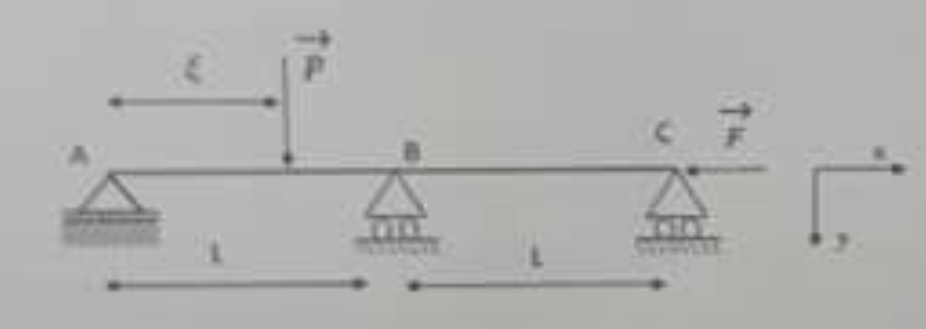
\includegraphics[width=0.5\textwidth]{ex1-1.png}
 \caption{}
 \label{fig:1}
\end{figure}

\subsection{Partie I}

Dans cette partie on étudie la structure par la théorie des poutres classiques sans se soucier d'une éventuelle instabilité.

\begin{enumerate}
 \item Calculer les réactions aux appuis A, B et C en choississant la réaction au point B comme inconnue hyperstatique (on utilise Castigliano et on ne garde que l'énergie de déformation due au moment fléchissant).
 \item Dessiner les diagrammes des efforts internes en indiquant les signes et les valeurs remarquables.
 \item Dessiner l'allure de la déformée de la structure sans effectuer les calculs, et préciser les points remarquables.
 \item Au lieu de la force concentrée \( P \), on considère maintenant une charge \( q \) \si{[N/m]} répartie uniformément sur la travée gauche (voir \figuref{2}). En utilisant la méthode de superposition, calculer le moment fléchissant au milieu de la travée gauche (en \( x = L/2 \)). Comparer la valeur à celle trouvée pour une force concentrée \( P \) dans le cas \( \xi = L/2 \) et \( P = qL \).
\end{enumerate}

\begin{figure}[!h]
 \centering
 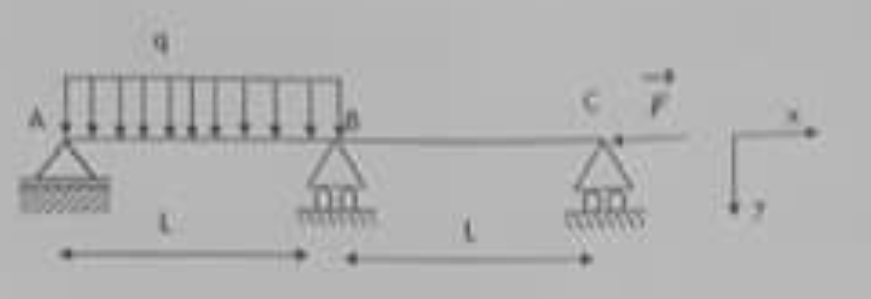
\includegraphics[width=0.5\textwidth]{ex1-2.png}
 \caption{}
 \label{fig:2}
\end{figure}

\begin{solution}

\subsection{Partie I}

\begin{enumerate}
 \item 
 
 On trace les forces de réaction aux appuis sur la \figuref{3}.
 
 \begin{solfig}{3}{Forces de réaction aux appuis}
 \centering
 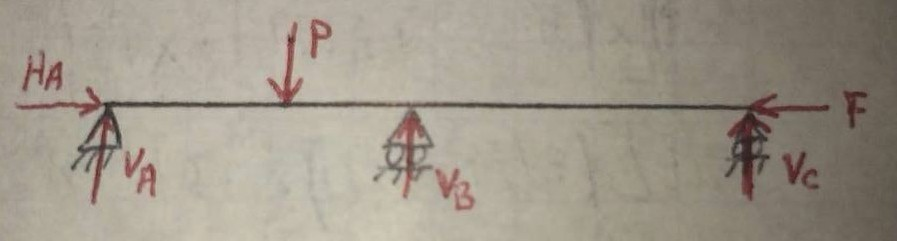
\includegraphics[width=0.5\textwidth]{ex1-3.jpg}
 \label{fig:3}
 \end{solfig}
 
 L'équilibre des forces et des moments donne:
 
 \[ \left\{ \begin{array}{rcl}
             H_A & = & F \\
             V_A + V_B + V_C & = & P \\
             P \xi & = & V_B L + 2 V_C L
            \end{array}
    \right. 
    \iff
    \left\{ \begin{array}{rcl}
             H_A & = & F \\
             V_A & = & P - \frac{1}{2} P \frac{\xi}{L} - \frac{1}{2} V_B \\
             V_C & = & \frac{1}{2} P \frac{\xi}{L} - \frac{1}{2} V_B
            \end{array}
    \right.
 \]
  
 On calcule ensuite les efforts internes le long de la poutre.
 
 \begin{itemize}
  \item \( 0 \le x \le \xi \) (\figuref{4})
  
  \begin{solfig}{4}{}
  \centering
  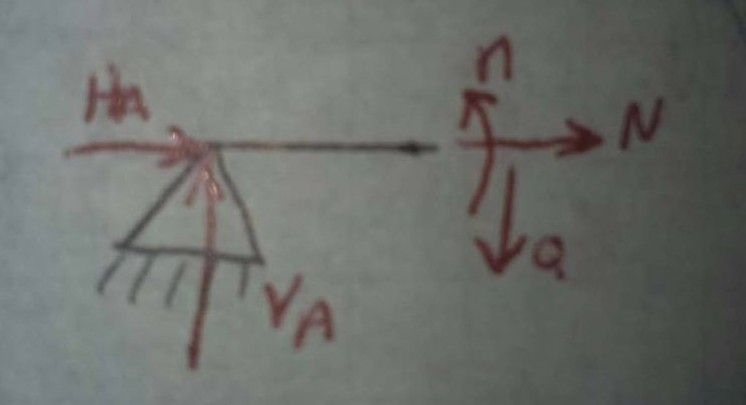
\includegraphics[width=0.3\textwidth]{ex1-4.jpg}
  \end{solfig}
  
  \[ \left\{ \begin{array}{rcl}
              N(x) & = & - H_A \\
              Q(x) & = & V_A \\
              M(x) & = & V_A x
             \end{array}
     \right.
     \implies
     \left\{ \begin{array}{rcl}
              N(x) & = & - F \\
              Q(x) & = & P - \frac{1}{2} P \frac{\xi}{L} - \frac{1}{2} V_B \\
              M(x) & = & \left( P - \frac{1}{2} P \frac{\xi}{L} - \frac{1}{2} V_B \right) x \implies \fpart{M}{V_B}(x) = -\frac{1}{2} x
             \end{array}
     \right.
  \]
  
  \item \( \xi \le x \le L \) (\figuref{5})
  
  \begin{solfig}{5}{}
  \centering
  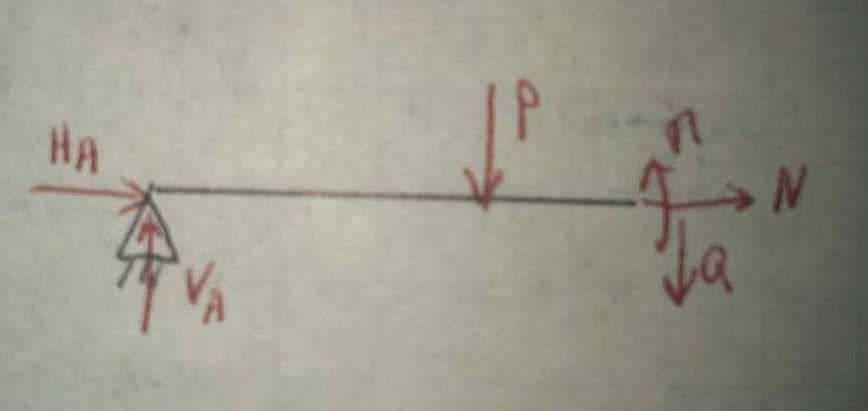
\includegraphics[width=0.3\textwidth]{ex1-5.jpg}
  \end{solfig}
  
  \[ \left\{ \begin{array}{rcl}
              N(x) & = & - H_A \\
              Q(x) & = & V_A - P \\
              M(x) & = & V_A x - P ( x - \xi)
             \end{array}
     \right.
     \implies
     \left\{ \begin{array}{rcl}
              N(x) & = & - F \\
              Q(x) & = & - \frac{1}{2} P \frac{\xi}{L} - \frac{1}{2} V_B \\
              M(x) & = & P \xi - P \frac{1}{2} \frac{\xi}{L} x - \frac{1}{2} V_B x \implies \fpart{M}{V_B}(x) = -\frac{1}{2} x
             \end{array}
     \right.
  \]
  
  \item \( L \le x \le 2L \) (\figuref{6})
  
  \begin{solfig}{6}{}
  \centering
  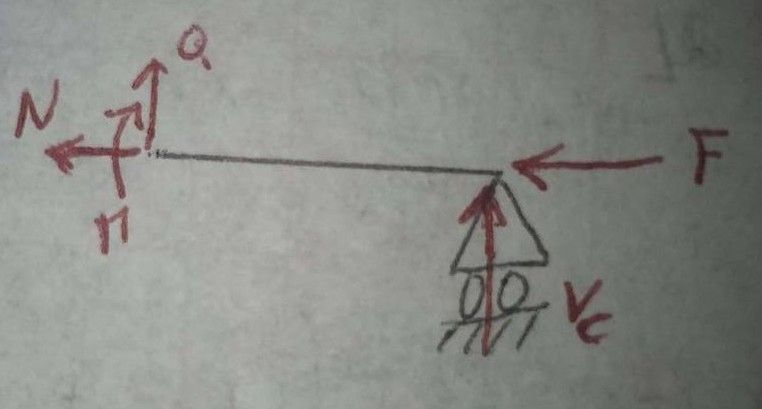
\includegraphics[width=0.3\textwidth]{ex1-6.jpg}
  \end{solfig}
  
  \[ \left\{ \begin{array}{rcl}
              N(x) & = & - F \\
              Q(x) & = & - V_C \\
              M(x) & = & V_C ( 2L - x )
             \end{array}
     \right.
     \implies
     \left\{ \begin{array}{rcl}
              N(x) & = & - F \\
              Q(x) & = & -\frac{1}{2} P \frac{\xi}{L} + \frac{1}{2} V_B \\
              M(x) & = & \left( \frac{1}{2} P \frac{\xi}{L} - \frac{1}{2} V_B \right) ( 2L - x ) \implies \fpart{M}{V_B}(x) = \frac{1}{2} ( x - 2L )
             \end{array}
     \right.
  \]
  
 \end{itemize}

 On utilise maintenant la méthode de Castigliano pour déterminer \( V_B \) (en utilisant uniquement l'énergie de déformation due au moment fléchissant):
 
 \[ \fpart{W}{V_B} = U_B \implies \int_0^{2L} M(x)\fpart{M}{V_B}(x) \, \dif x = 0 \,.\]
 
 En développant, on trouve ainsi
 
 \begin{align*}
  0 & = \int_0^\xi \left( V_A x \right) \left( -\frac{1}{2} x \right) \, \dif x + \int_\xi^L \left( V_A x - P ( x - \xi) \right) \left( -\frac{1}{2} x \right) \, \dif x + \int_L^{2L} \left( V_C ( 2L - x ) \right) \left( \frac{1}{2} ( x - 2L ) \right) \, \dif x \,, \\
  0 & = - \frac{1}{2} V_A \int_0^L x^2 \, \dif x + \frac{1}{2} P \int_\xi^L x ( x - \xi ) \, \dif x - \frac{1}{2} V_C \int_L^{2L} ( x - 2L )^2 \, \dif x \,, \\
  0 & = - \frac{1}{6} V_A L^3 + \frac{1}{2} P \left( \frac{1}{3} L^3 - \frac{1}{3} \xi^3 - \frac{1}{2} \xi L^2 + \frac{1}{2} \xi^3 \right) - \frac{1}{6} V_C L^3 \,, \\
  0 & = \frac{1}{6} L^3 \underbrace{\left( P - V_A - V_C \right)}_{V_B} + \frac{1}{2} P \left( \frac{1}{6} \xi^3 - \frac{1}{2} \xi L^2 \right) \,. \\
 \end{align*}

 La réaction au point B vaut finalement:
 
 \[ \boxed{ V_B = \frac{1}{2} P \left( 3 \left( \frac{\xi}{L} \right) - \left( \frac{\xi}{L} \right)^3 \right) } \,. \]
 
 Elle est positive pour tout \( \xi \) compris entre 0 et \( L \).
 
 Les réactions aux autres appuis valent
 
 \[ \left\{ \begin{array}{rcl}
             H_A & = & F \,, \\
             V_A & = & P \left( 1 - \frac{5}{4} \left( \frac{\xi}{L} \right) + \frac{1}{4} \left( \frac{\xi}{L} \right)^3 \right) \,, \\
             V_C & = & \frac{1}{4} P \left( \left( \frac{\xi}{L} \right)^3 - \left( \frac{\xi}{L} \right) \right) \,.
            \end{array}
    \right.
 \]
 
 \item 
 
 \begin{itemize}
  \item L'effort normal vaut
  
  \[ N(x) = - F \,, \qquad 0 \le x \le 2L \,. \]
  
  La seule valeur remarquables est \( - F \) (\figuref{graph1}).
  
  \begin{solfig}{graph1}{Effort normal}
    \begin{tikzpicture}[scale=0.7]
    \begin{axis}[
        axis x line=center,
        axis y line=left,
        xtick={0.5,1,2},
        xticklabels={$\xi$,$L$,$2L$},
        ytick={-1,1},
        yticklabels={$F$,$-F$},
        xlabel={$x$},
        ylabel={$y$},
        y axis line style = {stealth-},
        every axis x label/.style={at={(ticklabel* cs:1.05)},anchor=west,},
        every axis y label/.style={at={(ticklabel* cs:0)},anchor=north,},
        xmin=0,
        xmax=2.5,
        ymin=-2.5,
        ymax=2.5]
        \addplot[mark=*,color=red] coordinates {(0,1)(0.5,1)(1,1)(2,1)};
        \addplot[dashed,color=red] coordinates {(2,1)(2,0)};
    \end{axis}
    \end{tikzpicture}
  \end{solfig}
  
  \item L'effort tranchant vaut 
  
  \[ Q(x) = \left\{ \begin{array}{rcl}
              P \left( 1 - \frac{5}{4} \left( \frac{\xi}{L} \right) + \frac{1}{4} \left( \frac{\xi}{L} \right)^3 \right) & \,, & 0 \le x \le \xi \,. \\
              \frac{1}{4} P \left( \left( \frac{\xi}{L} \right)^3 - 5 \left( \frac{\xi}{L} \right) \right) & \,, & \xi \le x \le L \,. \\
              \frac{1}{4} P \left( \left( \frac{\xi}{L} \right) - \left( \frac{\xi}{L} \right)^3 \right) & \,, & L \le x \le 2L \,.
             \end{array}
     \right.
  \]
  
  Les troix valeurs remarquables sont données dans l'équation précédente (\figuref{graph2}).
  
  \begin{solfig}{graph2}{Effort tranchant}
    \begin{tikzpicture}[scale=0.7]
    \begin{axis}[
        axis x line=center,
        axis y line=left,
        xtick={0.5,1,2},
        xticklabels={$\xi$,$L$,$2L$},
        ytick={-1,1},
        yticklabels={$P$,$-P$},
        xlabel={$x$},
        ylabel={$y$},
        y axis line style = {stealth-},
        every axis x label/.style={at={(ticklabel* cs:1.05)},anchor=west,},
        every axis y label/.style={at={(ticklabel* cs:0)},anchor=north,},
        xmin=0,
        xmax=2.5,
        ymin=-1.5,
        ymax=1.5]
        \addplot[mark=*,color=red] coordinates {(0,-13/32)(0.5,-13/32)};
        \addplot[dashed,color=red] coordinates {(0.5,-13/32)(0.5,19/32)};
        \addplot[mark=*,color=red] coordinates {(0.5,19/32)(1,19/32)};
        \addplot[dashed,color=red] coordinates {(1,19/32)(1,-3/32)};
        \addplot[mark=*,color=red] coordinates {(1,-3/32)(2,-3/32)};
        \addplot[dashed,color=red] coordinates {(2,-3/32)(2,0)};
    \end{axis}
    \end{tikzpicture}
  \end{solfig}
  
  \item Le moment fléchissant vaut
  
  \begin{equation}
  \label{eq:1}
   M(x) = \left\{ \begin{array}{rcl}
              P x \left( 1 - \frac{5}{4} \left( \frac{\xi}{L} \right) + \frac{1}{4} \left( \frac{\xi}{L} \right)^3 \right) & \,, & 0 \le x \le \xi \,. \\
              P \left( \xi + x \left( - \frac{5}{4} \left( \frac{\xi}{L} \right) + \frac{1}{4} \left( \frac{\xi}{L} \right)^3 \right) \right) & \,, & \xi \le x \le L \,. \\
              \frac{1}{4} P \left( \left( \frac{\xi}{L} \right)^3 - \left( \frac{\xi}{L} \right) \right) (2 L -x ) & \,, & L \le x \le 2L \,.
             \end{array}
          \right.
  \end{equation}

  Les valeurs remarquables sont (\figuref{graph3})
  
  \[ \left\{ \begin{array}{rcl}
              M( x = \xi ) & = & P \xi \left( 1 - \frac{5}{4} \left( \frac{\xi}{L} \right) + \frac{1}{4} \left( \frac{\xi}{L} \right)^3 \right) \,, \\
              M( x = L ) & = & \frac{1}{4} P L \left( \left( \frac{\xi}{L} \right)^3 - \left( \frac{\xi}{L} \right) \right) \,.
             \end{array}
     \right.
  \]
  
  \begin{solfig}{graph3}{Moment fléchissant}
    \begin{tikzpicture}[scale=0.7]
    \begin{axis}[
        axis x line=center,
        axis y line=left,
        xtick={0.5,1,2},
        xticklabels={$\xi$,$L$,$2L$},
        ytick={-1,1},
        yticklabels={$PL$,$-PL$},
        xlabel={$x$},
        ylabel={$y$},
        y axis line style = {stealth-},
        every axis x label/.style={at={(ticklabel* cs:1.05)},anchor=west,},
        every axis y label/.style={at={(ticklabel* cs:0)},anchor=north,},
        xmin=0,
        xmax=2.5,
        ymin=-1.5,
        ymax=1.5]
        \addplot[mark=*,color=red] coordinates {(0,0)(0.5,-13/64)(1,3/32)(2,0)};
    \end{axis}
    \end{tikzpicture}
  \end{solfig}
  
 \end{itemize}

 
 \item La solution exacte est établie sur la \figuref{graph4}. Pour en obtenir une solution approchée,
 on se rappelle que le signe de la dérivée seconde de \( v(x) \) est le signe opposé de \( M(x) \).
 On voit bien que la concavité de la déformée est négative au niveau du point A, le moment fléchissant est alors positif.
 Ensuite, la concavité devient positive à partir d'un point \( \bar{x} \) compris entre \( \xi \) et \( L \), et cela jusqu'au bout de la poutre au point C.
 Ce résultat est logique puisque \( M(x) \) devient négatif à cet endroit \( \bar{x} \).
 
 On peut également noter que la déformée et la dérivée de la déformée sont continues en \( x = \xi \)\footnote{On pourrait finalement préciser que la déformée est nulle en \( x = 0, x = L \) et \( x = 2 L \)\dots}.

 
   \begin{solfig}{graph4}{Allure de la déformée}
    \begin{tikzpicture}[scale=0.7]
    \begin{axis}[
        axis x line=center,
        axis y line=left,
        xtick={0.5,1,2},
        xticklabels={$\xi$,$L$,$2L$},
        ytick={0},
        yticklabels={,,},
        xlabel={$x$},
        ylabel={$y$},
        y axis line style = {stealth-},
        every axis x label/.style={at={(ticklabel* cs:1.05)},anchor=west,},
        every axis y label/.style={at={(ticklabel* cs:0)},anchor=north,},
        xmin=0,
        xmax=2.5,
        ymin=-0.5,
        ymax=0.5]
        \addplot[red,domain=0:0.5]{10*13/192*(x^3-9/13*x)};
        \addplot[red,domain=0.5:1]{-10*(-1/48+1/48*x+(29*x-48*x^2+19*x^3)/192)};
        \addplot[red,domain=1:2]{-10*(6-11*x+6*x^2-x^3)/64};
    \end{axis}
    \end{tikzpicture}
  \end{solfig}
  
 \item 
 
 Au lieu de recommencer les calculs depuis le début, on tire profit du fait que ce nouveau problème est très semblable au problème précedent. En effet, il suffit de considérer que la charge \( q \) est une somme infinie de forces ponctuelles infinitésimales \( q \dif \xi \) situées entre \( x = 0 \) et \( x = L \). Le principe de superposition stipule que l'on peut décomposer un problème complet (celui avec la charge \( q \)) en plusieurs sous-problèmes pour lesquels la  combinaison des conditions limites reconduit au problème général. On peut alors trouver la solution\footnote{Dans notre cas, c'est le moment fléchissant en \( x = L/2 \).} dans chaque sous-problème et ensuite les sommer pour avoir la solution du problème général.
 
 Donc, on calcule la solution du sous-problème, notée \( \dif M_q(L/2) \), due à une force ponctuelle infinitésimale \( q \dif \xi \) en \( x = \xi \). C'est exactement ce qu'on a résolu aux points précédents, en remplaçant la force \( P \) par \( q \dif \xi \). On reprend donc simplement les résultats de l'Équation~\ref{eq:1}:
 
 \[ 
       \dif M_q(x) =  \left\{ 
                            \begin{array}{rcl}
                                q x \left( 1 - \frac{5}{4} \left( \frac{\xi}{L} \right) + \frac{1}{4} \left( \frac{\xi}{L} \right)^3 \right) \dif \xi & \,, & 0 \le x \le \xi \,. \\
                                q \left( \xi + x \left( - \frac{5}{4} \left( \frac{\xi}{L} \right) + \frac{1}{4} \left( \frac{\xi}{L} \right)^3 \right) \right) \dif \xi & \,, & \xi \le x \le L \,.
                            \end{array}
                        \right.
 \]
 
 On l'évalue en \( x = L/2 \),
 
 \[ 
       \dif M_q(L/2) =  \left\{ 
                            \begin{array}{rcl}
                                \frac{1}{8} q L \left( 3 \left( \frac{\xi}{L} \right) + \left( \frac{\xi}{L} \right)^3 \right) \dif \xi & \,, & 0 \le \xi \le L/2 \,. \\
                                \frac{1}{2} q L \left( 1 - \frac{5}{4} \left( \frac{\xi}{L} \right) + \frac{1}{4} \left( \frac{\xi}{L} \right)^3 \right) \dif \xi & \,, & L/2 \le \xi \le L \,.
                            \end{array}
                        \right.
 \]
 
 Il est utile de remarquer que si \( 0 \le \xi \le L/2 \), il faut utiliser la deuxième relation (donnant le moment fléchissant pour \( \xi \le x \le L \)) puisque \( L/2 \) se situe dans cet intervalle. On établit une remarque similaire pour \( L/2 \le \xi \le L \).
 
 Il ne reste plus qu'à intégrer\footnote{C'est-à-dire sommer les solutions de tous les sous-problèmes.} cette relation entre \( \xi = 0 \) et \( \xi = L \) pour trouver le moment fléchissant en \( x = L/2 \) dû à une charge répartie \( q \) entre \( x = 0 \) et \( x = L \).
 
 \begin{align*}
   M_q(L/2) & = \int \dif M_q(L/2) \,, \\
   & = \int_0^{L/2} \frac{1}{8} q L \left( 3 \left( \frac{\xi}{L} \right) + \left( \frac{\xi}{L} \right)^3 \right) \dif \xi + \int_{L/2}^{L} \frac{1}{2} q L \left( 1 - \frac{5}{4} \left( \frac{\xi}{L} \right) + \frac{1}{4} \left( \frac{\xi}{L} \right)^3 \right) \dif \xi \,, \\
   & = \frac{1}{8} q L^2 \int_0^{1/2} \left( 3 \eta + \eta^3 \right) \dif \eta + \frac{1}{8} q L^2 \int_{1/2}^{1} \left( 4 - 5 \eta + \eta^3 \right) \dif \eta \,, \\
   & = \frac{25}{512} q L^2 + \frac{23}{512} q L^2 \,,
 \end{align*}
 
 \[ \boxed{M_q(L/2) = \frac{3}{32} q L^2} \,, \]
 
 en utilisant le changement de variable \( \eta = \xi / L \).
 
 On peut comparer cette valeur à celle obtenue pour une force ponctuelle \( q L \) en \( \xi = L/2 \). On reprend la première ligne de l'Équation~\ref{eq:1},
 
 \[ M_P(L/2) = P x \left( 1 - \frac{5}{4} \left( \frac{\xi}{L} \right) + \frac{1}{4} \left( \frac{\xi}{L} \right)^3 \right) \,, \]
 
 en remplaçant \( P \) par \( q L \), \( x \) par \( L/2 \) et \( \xi \) par \( L/2 \) pour trouver
 
 \[ \boxed{M_P(L/2) = \frac{13}{64} q L^2} \,. \]
 
 Ce moment fléchissant représente plus du double de celui dû à la charge répartie \( q \), ce résultat est logique puisque la charge répartie contribue de moins en moins au fur et à mesure qu'elle s'éloigne du centre de la travée gauche\footnote{Il y a même une contribution nulle aux extrémités de la charge, en \( \xi = 0 \) et en \( \xi = L \).}.
 
\end{enumerate}

\end{solution}

\end{document}
